\documentclass[11pt,letterpaper]{article}
\usepackage[top=3cm, bottom=2cm, left=2cm, right=2cm, columnsep=20pt]{geometry}
\usepackage{pdfpages}
\usepackage{graphicx}
\usepackage{etoolbox}
\apptocmd{\sloppy}{\hbadness 10000\relax}{}{}
\usepackage[numbers]{natbib}
\usepackage[T1]{fontenc}
\usepackage{ragged2e}
\usepackage[french]{babel}
\usepackage{listings}
\usepackage{color}
\usepackage{soul}
\usepackage[utf8]{inputenc}
\usepackage[export]{adjustbox}
\usepackage{caption}
\usepackage{amsmath}
\usepackage{amssymb}
\usepackage{float}
\usepackage{csquotes}
\usepackage{fancyhdr}
\usepackage{wallpaper}
\usepackage{siunitx}
\usepackage[indent]{parskip}
\usepackage{textcomp}
\usepackage{gensymb}
\usepackage{multirow}
\usepackage[hidelinks]{hyperref}
\usepackage{abstract}
\usepackage{svg}
\usepackage{multicol}
\usepackage{subcaption}


\renewcommand{\abstractnamefont}{\normalfont\bfseries}
\renewcommand{\abstracttextfont}{\normalfont\itshape}
\usepackage{titlesec}
\titleformat{\section}{\large\bfseries}{\thesection}{1em}{}
\titleformat{\subsection}{\normalsize\bfseries}{\thesubsection}{1em}{}
\titleformat{\subsubsection}{\normalsize\bfseries}{\thesubsubsection}{1em}{}

\usepackage{xcolor}
\definecolor{codegreen}{rgb}{0,0.6,0}
\definecolor{codegray}{rgb}{0.5,0.5,0.5}
\definecolor{codepurple}{rgb}{0.58,0,0.82}
\definecolor{backcolour}{rgb}{0.95,0.95,0.92}
\lstdefinestyle{mystyle}{
    backgroundcolor=\color{backcolour},   
    commentstyle=\color{codegreen},
    keywordstyle=\color{magenta},
    numberstyle=\tiny\color{codegray},
    stringstyle=\color{codepurple},
    basicstyle=\ttfamily\footnotesize,
    breakatwhitespace=false,         
    breaklines=true,                 
    captionpos=b,                    
    keepspaces=true,                 
    numbers=left,                    
    numbersep=5pt,                  
    showspaces=false,                
    showstringspaces=false,
    showtabs=false,                  
    tabsize=2
}
\lstset{style=mystyle}

\usepackage[most]{tcolorbox}
\newtcolorbox{note}[1][]{
  enhanced jigsaw,
  borderline west={2pt}{0pt}{black},
  sharp corners,
  boxrule=0pt, 
  fonttitle={\large\bfseries},
  coltitle={black},
  title={Note:\ },
  attach title to upper,
  #1
}

%----------------------------------------------------

\setlength{\parindent}{0pt}
\DeclareCaptionLabelFormat{mycaptionlabel}{#1 #2}
\captionsetup[figure]{labelsep=colon}
\captionsetup{labelformat=mycaptionlabel}
\captionsetup[figure]{name={Figure }}
\captionsetup[table]{name=Tableau}
\newcommand{\inlinecode}{\normalfont\texttt}
\usepackage{enumitem}
\setlist[itemize]{label=\textbullet}

\begin{document}
\begin{titlepage}
\center

\begin{figure}
    \ThisULCornerWallPaper{.4}{Polytechnique_signature-RGB-gauche_FR.png}
\end{figure}
\vspace*{2 cm}

\textsc{\Large \textbf{PHS3910 --} Techniques expérimentales et instrumentation}\\[0.5cm]
\large{\textbf{Équipe : Lundi 03}}\\[1.5cm]

\rule{\linewidth}{0.5mm} \\[0.5cm]
\Large{\textbf{Suivi de particules}} \\[0.2cm]
\text{Fiche technique}\\
\rule{\linewidth}{0.5mm} \\[2.3cm]

\large{\textbf{Présenté à}\\
  Jean Provost\\
  Lucien Weiss\\[2.5cm]
  \textbf{Par :}\\
  Émile \textbf{Guertin-Picard} (2208363)\\
  Philippine \textbf{Beaubois} (2211153)\\
  Marie-Lou \textbf{Dessureault} (2211129)\\
  Maxime \textbf{Rouillon} (2213291)\\[3cm]}

\large{\today\\
Département de Génie Physique\\
Polytechnique Montréal\\}

\end{titlepage}

%----------------------------------------------------

\tableofcontents
\pagenumbering{roman}
\newpage

\pagestyle{fancy}
\setlength{\headheight}{14pt}
\renewcommand{\headrulewidth}{0pt}
\fancyfoot[R]{\thepage}

\pagestyle{fancy}
\fancyhf{}
\renewcommand{\headrulewidth}{1pt}
\fancyhead[L]{\textbf{PHS3910}}
\fancyhead[C]{Fiche technique : suivi de particules}
\fancyhead[R]{\today}
\fancyfoot[R]{\thepage}

\pagenumbering{arabic}
\setcounter{page}{1}

%----------------------------------------------------

\section{Description générale et spécifications}

Cette fiche technique, à la demande du Gouvernement du Québec, présente les caractéristiques 
d'un dispositif de mesure de taille de microparticules contaminant l'environnement près de 
l'usine Polyfab. Les composantes principales sont un laser 405 nm (CPS405)
pour illuminer les fluorophores dans les échantillons, un objectif de microscope (grossissement 
$M = 20$, aperture NA $= 0.4$), puis une lentille tube de 150 mm de focale
(LA1433-A-ML) pour converger les rayons sortants de l'objectif sur le capteur d'une caméra CMOS 
(CS165MU) pour l'analyse \cite{noauthor_thorlabs_2024}. Ce système présente une résolution
théorique de 1.012 µm \cite{rouillon_travail_2024}. Afin d'analyser des particules d'environ cette taille, un traitement
numérique est fait pour extraire la taille des particules du mouvement brownien filmé, avec 
une résolution sous-pixellaire. Avec ce procédé, l'appareil a été testé pour des tailles de 
particules dans la plage 1-10 µm. Suite à la caractérisation de particules 
de 1 µm, la valeur identifiée est de 1.6 $\pm$ 0.3 µm.
Pour la caractérisation de particules de 10 µm, elle est de 6 $\pm$ 1 µm. Le système, monté sur table optique et utilisable dans le noir 
seulement, a des dimensions de $600 \times 90 \times 200$ mm, tel que présenté à 
la figure \ref{schema_micro}. La résolution de l'appareil post-traitement est de 0.3 µm, et
son grossissement réel est de $17.14 \pm 0.02$. Sans compter la table optique, le dispositif a pour coût total 1789.39 \$, prix qui
peut être réduit par l'usage d'impression 3D. Les spécifications du dispositif sont rassemblées dans le
tableau \ref{specs} ci-dessous.

\begin{figure}[H]
  \centering
  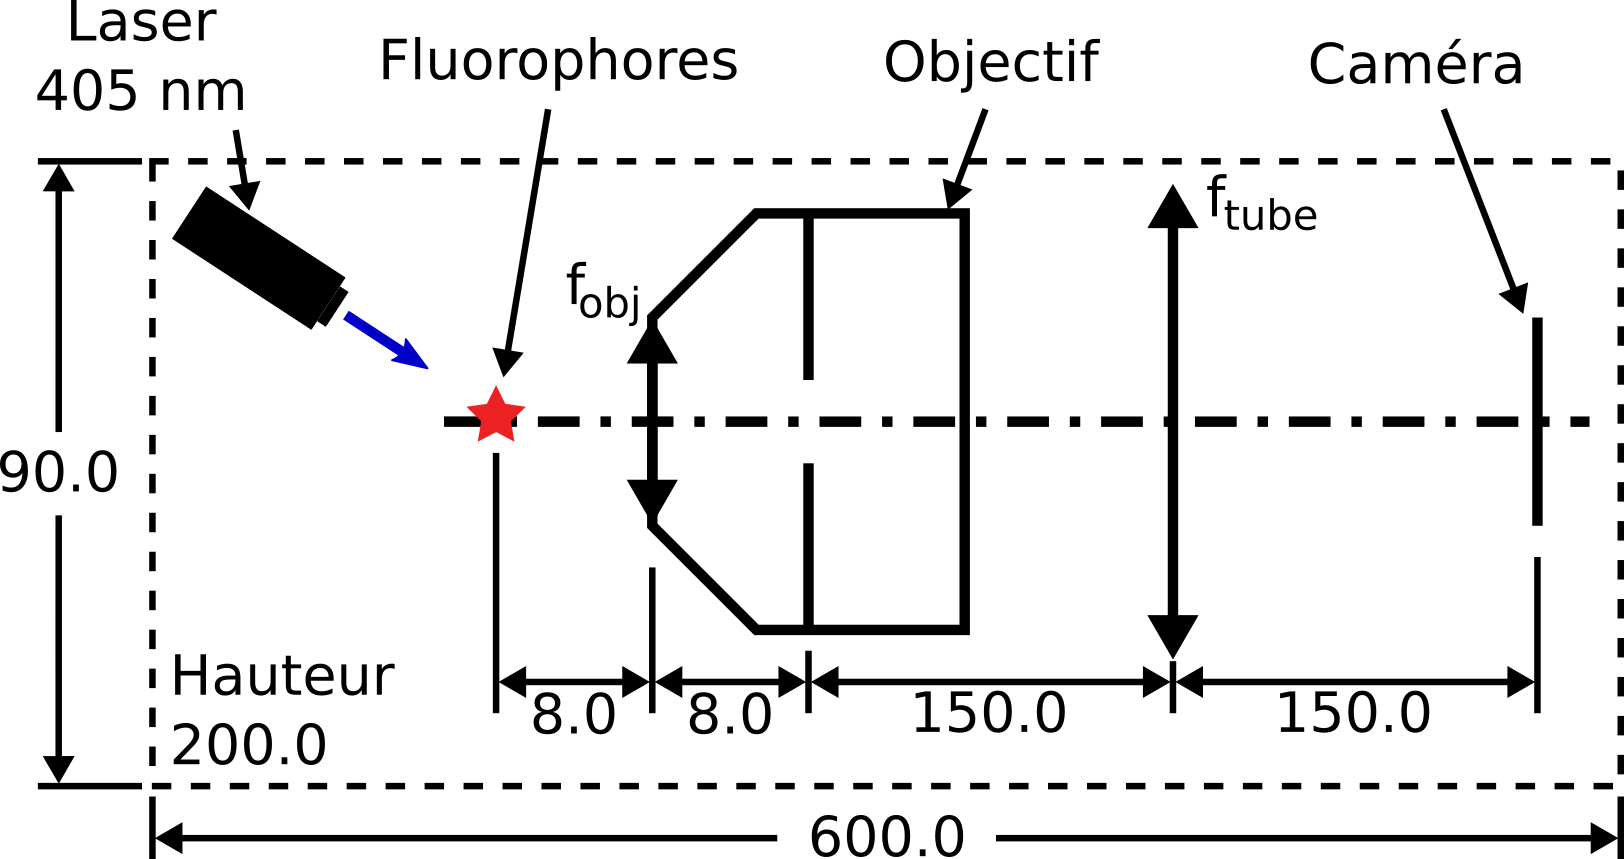
\includegraphics[scale=2.8]{schema_fiche_tech.png}
  \caption{Schéma du microscope avec les dimensions critiques. Toutes les dimensions sont en millimètres avec une tolérance de $\pm$ 1 mm.}
  \label{schema_micro}
\end{figure}

\begin{table}[H]
  \centering
  \caption{Tableau des spécifications}
  \begin{tabular}{|p{2.5cm}|p{2cm}|p{3cm}|p{1.5cm}|p{6.5cm}|}
  \hline
      Magnification réelle & Résolution ($\mu m$) & Dimensions (mm) & Coût  \$CAD & Composantes \\ \hline\hline
      $17.14\pm0.02$ & 0.3 & L 600 $\times$ W 90 $\times$ H 200 & \$1789.39 & \vspace{-20pt} {\small\parbox{7cm}{\setlength{\columnsep}{0pt} 
      \begin{multicols}{2}\begin{itemize}[label=$\triangleright$, topsep=0pt, itemsep=0pt]
            \item KM100S
            \item CS165MU
            \item 420FDL12
            \item LA1433-A-ML
            \item CPS405
            \item LMR1
            \item TR3-P5
            \item PH4
            \item PH3
            \item BA1
            \item BA1S
            \item BA2 
            \item VC1 
        \end{itemize}
      \end{multicols} } } \\ \hline
  \end{tabular}
  \label{specs}
\end{table}




\section{Rapports de tests}

Cette section explique en détail le processus et les résultats pour les tests de caractérisation
effectués sur le dispositif de suivi de particules.

\subsection{Suivi de particules}

Pour obtenir la taille d'une particule avec la plus grande précision possible, l'analyse de son
mouvement brownien est utilisée. La position de la particule doit être 
déterminée sur au moins une cinquantaine d'instants successifs, avant de pouvoir procéder à l'estimation de son 
coefficient de diffusion et de sa taille. Des images sont prises pour chaque instant.

Pour positionner la particule avec la plus faible incertitude possible, un 
\textit{fit} gaussien est effectué sur l'image pixelisée de la particule pour un moment précis. Pour que le \textit{fit} s'effectue
adéquatement, il faut restreindre la zone de \textit{fit} à la particule. Pour ce faire, le suivi de la particule commence 
autour de la position précédente de la particule, par la recherche de maxima d'intensité surpassant un seuil. Les
dimensions de la zone rectangulaire en question et le seuil utilisé sont des valeurs déterminées par essai-erreur
et sont respectivement d'environ 100 pixels de côté et une intensité de 50 sur un maximum de 255.
Une fois le nombre de maxima obtenu, soit le nombre de particules potentielles, la zone de \textit{fit} est recentrée sur 
la particule la plus similaire à celle du départ.  

Pour reconnaitre la particule, un système de comparaison des particules potentielles en fonction de leur taille 
et leur luminosité est utilisé lorsque plus d'une particule est dans la même zone. 
La taille, soit le nombre de pixels au-dessus d'un seuil fixé, y a un rôle prépondérant, mais la luminosité, soit 
la moyenne d'intensité des pixels en question, a également un impact. Ces informations sont obtenues en centrant 
l'image sur la particule d'intérêt et en appliquant la\ fonction \texttt{DBSCAN} pour regrouper les maximas en des entités
qui correspondent aux particules. La luminosité et la taille obtenues sont alors comparées à la luminosité et la 
taille de la première observation qui sert de référence. La première observation est obtenue comme les suivantes,
avec comme seul différence que sa détection est faite par l'humain utilisant le système, qui clique initialement 
sur la particule que le système aura à suivre.

Une fois que la particule peut être suivie d'un instant au suivant, la localisation de la particule est obtenue à 
l'aide du \textit{fit} gaussien, et l'incertitude sur la position correspond alors à l'écart-type de la gaussienne obtenue, 
qui est généralement plus faible que la taille d'un pixel. 
Des vérifications sont faites pour s'assurer que la nouvelle position est plausible et elle est alors
enregistrée avant de servir de référence pour le traitement du cadre suivant.

Si la particule choisie sort de l'écran avant la fin des instants observés, le système s'arrête tout simplement à 
sa dernière position identifiable, soit environ 100 pixels avant le bord.

\subsection{Paramètres utilisés \label{para}}
Certains paramètres du dispositif ont eu besoin d'être choisis pour optimiser sa performance. Entre autres,
l'objectif du microscope choisi possède une magnification théorique de 20, et une ouverture numérique de 0.4. Après quelques essais, 
il a été conclu qu'une magnification de 20 offrait une plage de fonctionnement optimale, en considérant 
que pour des magnifications plus élevées, les plus grosses particules (de l'ordre de 10 microns) se déplaçaient souvent hors de la région observée. 
La figure \ref{exposition} ci-dessous présente les images
capturées pour trois différents temps d'exposition.

\begin{figure}[H]
  \begin{subfigure}{0.3\textwidth}
      \centering
      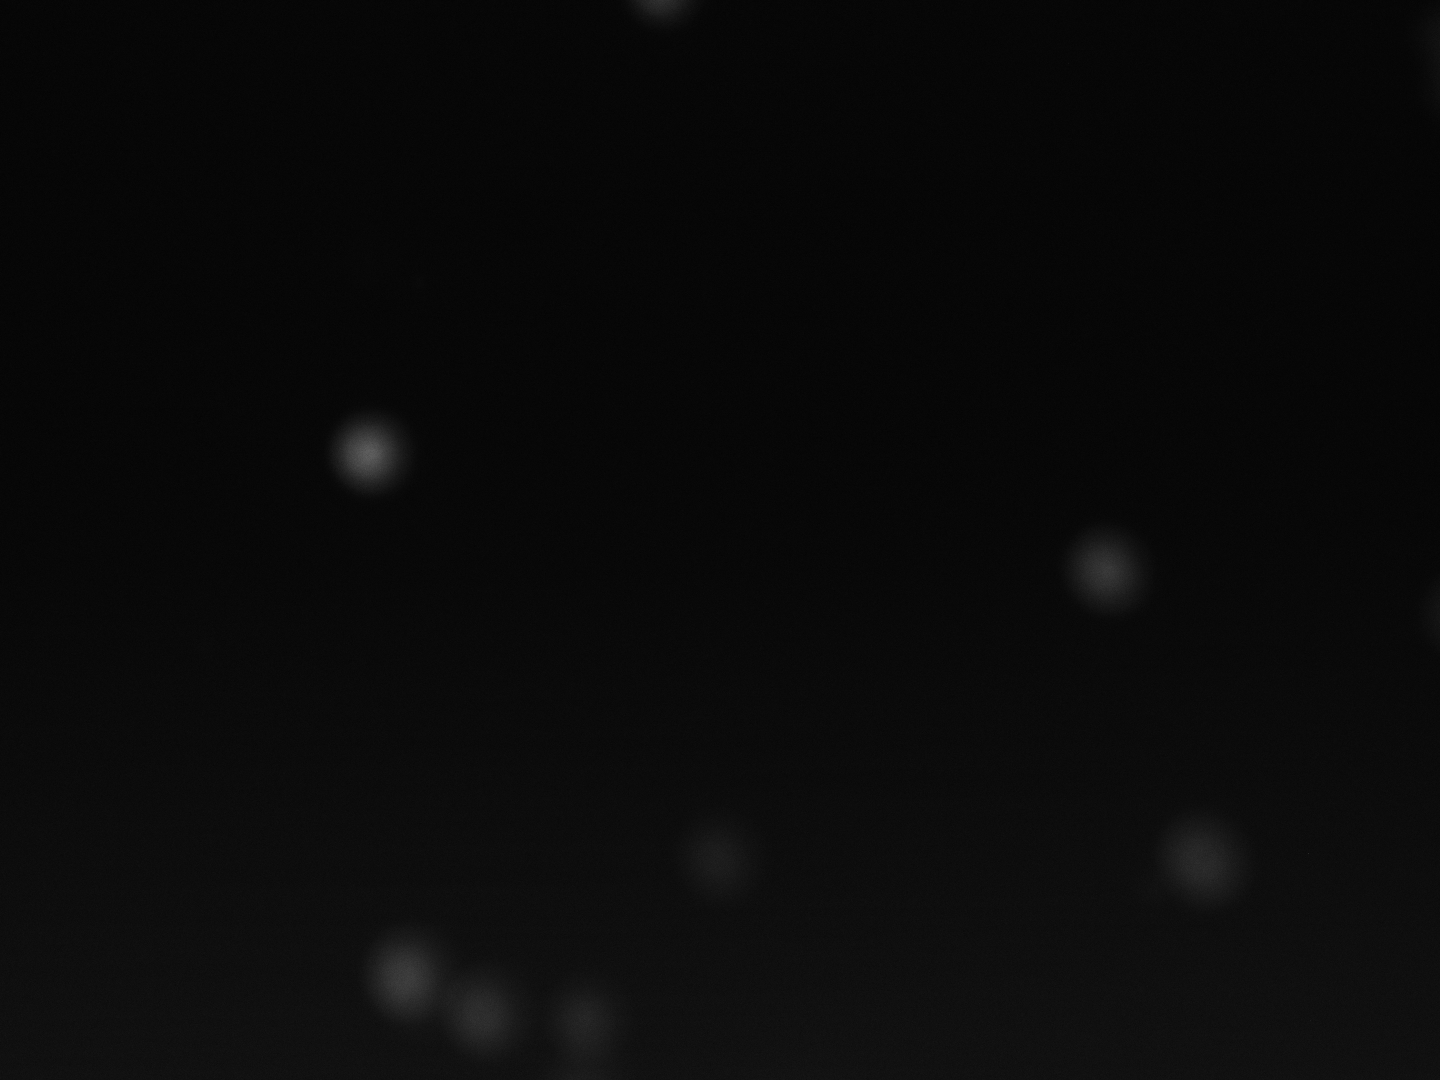
\includegraphics[width=\textwidth]{essai_10um_2im_50ms.png}
      \caption{}
      \label{a}
  \end{subfigure}
  \hfill
  \begin{subfigure}{0.3\textwidth}
      \centering
      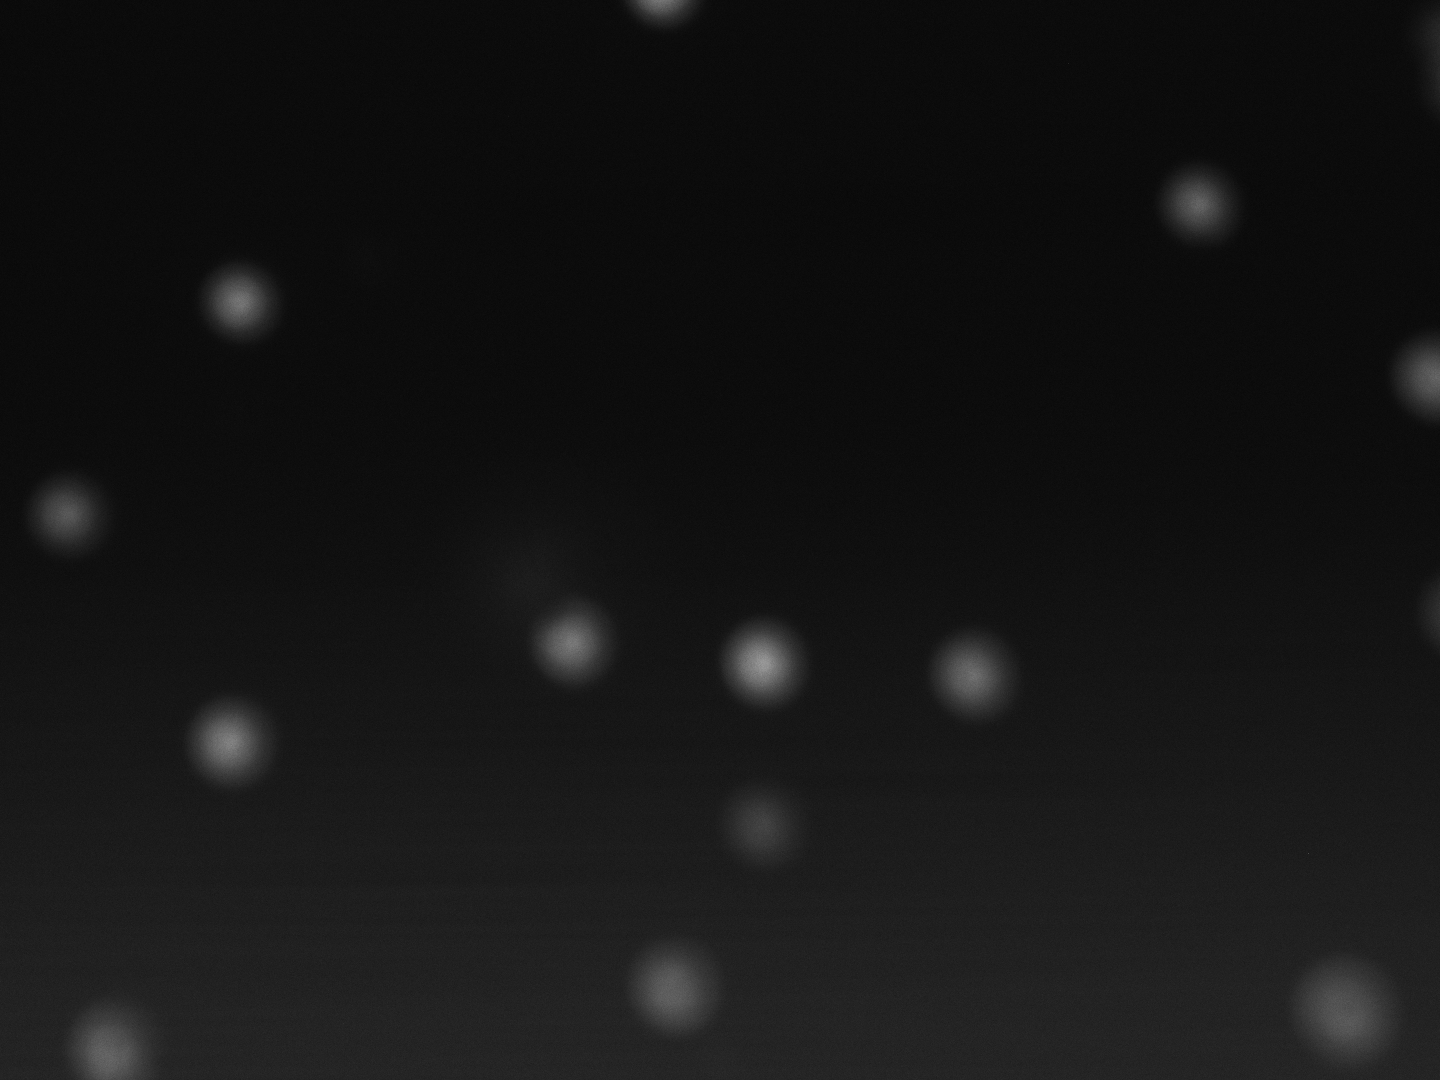
\includegraphics[width=\textwidth]{essai_10um_2im_100ms.png}
      \caption{}
      \label{b}
  \end{subfigure}
  \hfill
  \begin{subfigure}{0.3\textwidth}
    \centering
    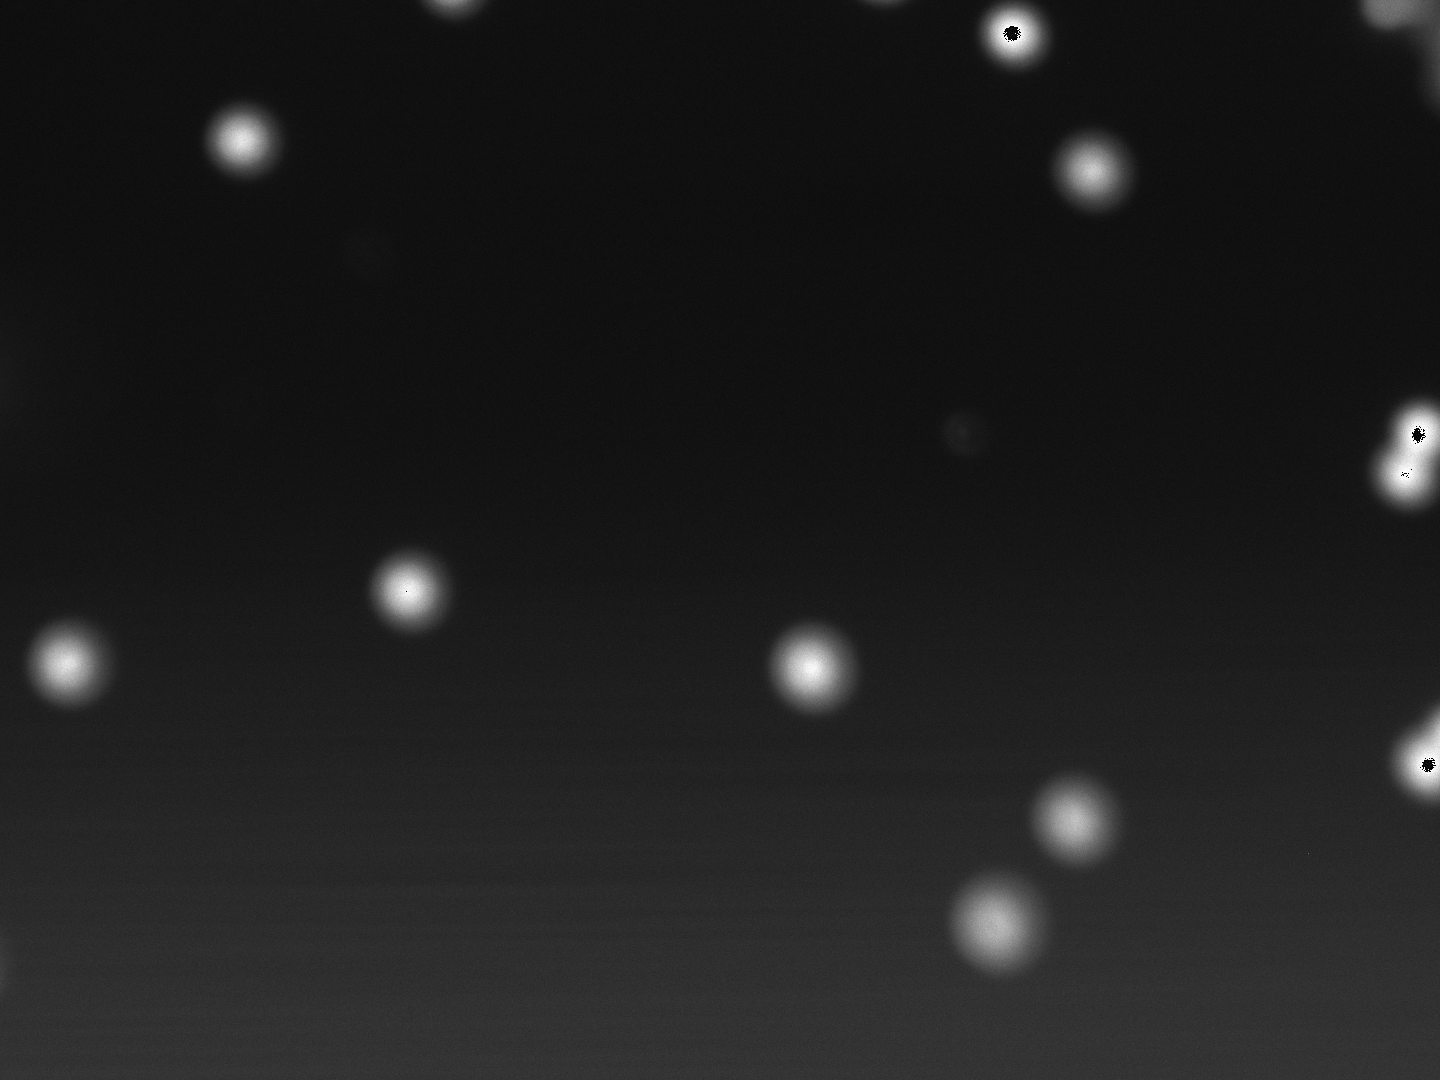
\includegraphics[width=\textwidth]{essai_10um_1im_150ms.png}
    \caption{}
    \label{c}
  \end{subfigure}
  \caption{Image capturée pour un temps d'exposition de: (a) 50 ms (b) 100 ms et (c) 150 ms.}
      \label{exposition}
\end{figure}
Ici, l'image \ref{a} est sous-exposée et l'image \ref{c} est surexposée. Pour le cas sous-exposé, le contraste entre
le bruit et les particules est réduit, ce qui peut affecter la justesse des \textit{fits} gaussiens effectués pour suivre
le déplacement des particules. Pour le cas surexposé, l'intensité des pixels de certaines particules est saturée, ce qu'on peut
observer en haut à droite de l'image \ref{c}. Par conséquent, un temps d'exposition de 100 ms, correspondant à l'image \ref{b}, a été choisi.

La fréquence d'images $f_{image}$ est dépendante au temps d'exposition choisi. Effectivement, celle-ci doit respecter la contrainte
ci-dessous:
\begin{equation*}
  f_{image}\leq \frac{1}{\Delta t},
\end{equation*}
où $\Delta t$ correspond au temps d'exposition. Pour un temps d'exposition de 0.100 s, on a : $f_{image}\leq 1/0.100 = 10$ images/s. 
Normalement, la fréquence d'images peut être gardée à sa valeur maximale, mais après quelques essais, il a pu été observé que de nombreuses
images ne se sauvegardaient pas. Sachant que la position dans le temps de chaque capture d'image est importante pour le calcul de la MSD, la fréquence 
d'images a été réduite à deux images par secondes pour essayer de limiter le nombre d'images perdues. 

Afin d'obtenir un calcul des premiers points de la MSD ayant des poids statistiques significatifs, le nombre d'images capturées a été posé à 75. 
Ce choix a été fait pour que le nombre d'images enregistrées soit de 50 ou plus, en ajoutant une marge de 25 images pour prendre en compte les images qui seront 
potentiellement perdues.


\subsection{Magnification réelle}
La magnification réelle du système a été déterminée à l'aide d'une cible ayant des dimensions connues. L'image de la cible, capturée par la
caméra et suite au microscope, est présentée dans la figure \ref{cible}. La distance réelle entre le centre de deux carrés blancs voisins dans le 
quadrillage est de 0.01 mm.
\begin{figure}[H]
  \centering
  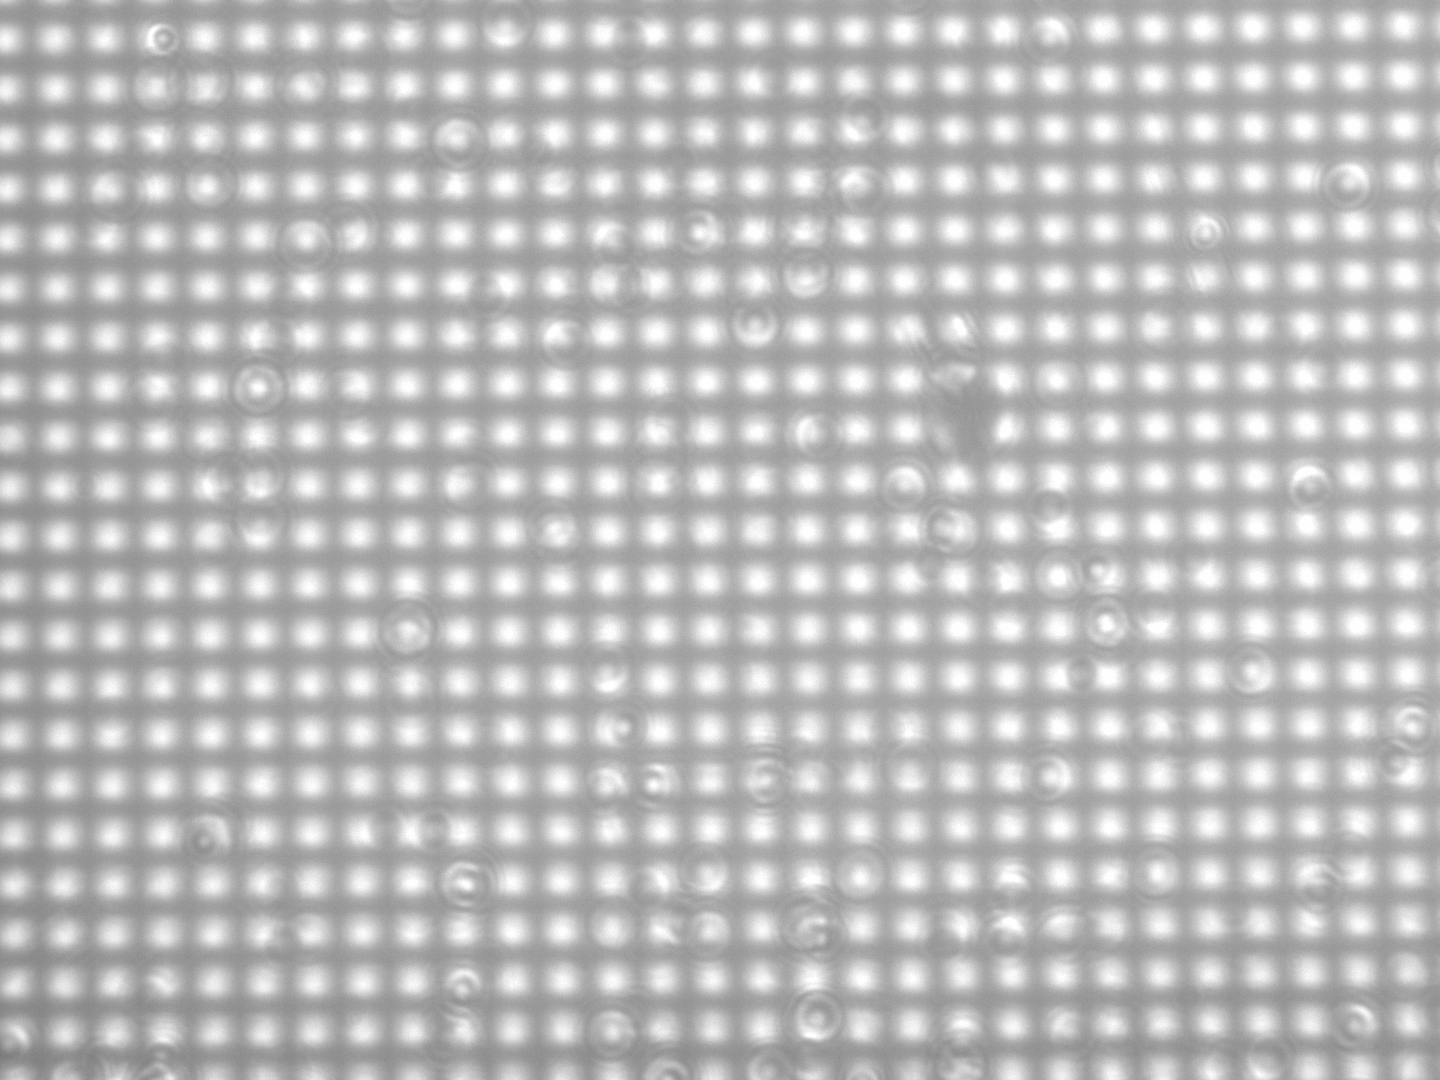
\includegraphics[scale=0.2]{magnification_rele.png}
  \caption{Image de la cible au plan du capteur.}
  \label{cible}
\end{figure}
Afin de déterminer la distance entre les centres pour l'image de la cible, deux \textit{fits} gaussiens ont
été effectués sur une région recadrée de l'image, comprenant l'équivalent de deux carrés blancs. L'image recadrée est illustrée dans la 
figure \ref{crop} ci-dessous.
\begin{figure}[H]
  \centering
  
\includegraphics[scale=2]{magnification_rele_crop.png}
  \caption{Image recadrée de la cible.}
  \label{crop}
\end{figure}
Les deux \textit{fits} gaussiens 2D ont été effectués avec la fonction Python \texttt{curve\_fit} sur la moitié droite et sur la moitié gauche de l'image \ref{crop},
ce qui a permis de trouver le centre de chaque carré blanc. La gaussienne 2D est décrite par:
\begin{equation}
  f(x,y)=A\cdot exp\left(-\left(\frac{(x-x_0)^2}{2\sigma_x^2}+\frac{(y-y_0)^2}{2\sigma_y^2}\right)\right)+B,
\end{equation}
où $A$ est l'amplitude, $B$ est le décalage, $x_0$ et $y_0$ sont les moyennes et $\sigma_x$ et $\sigma_y$ sont les écarts-types.
En ayant obtenu les coordonnées des centres des deux gaussiennes, on peut trouver la distance $d_{im}$ entre les deux centres:
\begin{equation}
  d_{im}=(x_{0_2}-x_{0_1})\cdot d_{pixel}\approx 0.1714 \text{ mm},
\end{equation}
où $d_{pixel}=3.45\times10^{-6}$ m est la dimension d'un pixel \cite{noauthor_thorlabs_2024-1}. Ici, on approxime la distance en utilisant la distance en $x$
parce que la composante $|y_{0_2}-y_{0_1}|\approx 0.6$ pixel est négligeable. Finalement, on retrouve la magnification réelle de l'objectif:
\begin{equation}
  m=\frac{d_{im}}{d_{vraie}}\approx\frac{0.1714}{0.01}= 17.14.
\end{equation}
L'incertitude sur $m$ provient des incertitudes sur les paramètres du \textit{fit} gaussien. 
On retrouve:
\begin{equation}
  \sigma_m=\frac{\sqrt{(d_{pixel}*\sigma_{x_{0_2}})^2+(d_{pixel}*\sigma_{x_{0_2}})^2}}{d_{vraie}}\approx0.0169.
\end{equation}
On obtient donc que la magnification réelle est de: $17.14\pm0.02$. Celle-ci permettra de redimensionner les images d'une échelle en pixel à une échelle métrique.

% Source caméra :

\subsection{Caractérisation de la taille de particules}

Lors de l'acquisition, il a été observé que la caméra ne parvient
pas à enregistrer chaque image. Afin de remedier ce problème, l'acquisition d'images remplace les images qui ne sont pas enregistrées par une image noire. 
Pour traiter les images et suivre les particules correctement, toutes les images noires sont premièrement ignorées pour 
produire une liste de positions. Les images de départ sont évaluées une par une, et à chaque fois qu'une
image noire apparaît, un vecteur \texttt{[NaN, NaN]} est ajouté à la liste contenant toutes les positions.
Cette procédure nous permet de savoir avec exactitude les temps des images qui n'ont pas pu être enregistrées. Une fois la liste de positions 
complétée, il est possible d'effectuer le calcul de la MSD avec la formule suivante: 
 \begin{align}
  MSD &= \frac{1}{N_{\Delta t}} \sum_{i=0}^{N_{\Delta t} - 1} \left( \mathbf{r}(i+\Delta t) - \mathbf{r}(i) \right)^2,\\ 
  \mathbf{r}(i) &= x(i)\hat{x}+ y(i)\hat{y}
\end{align}
où $N_{\Delta t}$ est le nombre de paires $i$ disponibles pour un intervalle $\Delta t$ et $\Delta t$ qui varie de 1 jusqu'au nombre de positions (nombre d'images) moins une. 
L'incertitude sur ces valeurs est donnée par la formule suivante: 
\begin{equation}
  \alpha =A+B
\end{equation}
\begin{align*}
  A = \sqrt{
    \begin{aligned}
      &\left( 2(x(i+\Delta t) - x(i))\cdot \Delta x(i+\Delta t) \right)^2 \\
      &+ \left( 2(x(i+\Delta t) - x(i))\cdot \Delta x(i) \right)^2
    \end{aligned}
  }
\end{align*}
\begin{align*}
  B = \sqrt{
    \begin{aligned}
      &\left( 2(y(i+\Delta t) - y(i))\cdot \Delta y(i+\Delta t) \right)^2 \\
      &+ \left( 2(y(i+\Delta t) - y(i))\cdot \Delta y(i) \right)^2.
    \end{aligned}
  }
\end{align*}

On remarque que c'est ici que le traitement de toutes les images est important, même celles qui ont été perdues, car sinon le $\Delta t$ n'aurait pas été cohérent avec la procédure de la MDS. 
La façon de traiter ce calcul avec les vecteurs $\left [ NaN ,NaN \right ]$ tout en perdant le moins d'information possible a été de définir que 
dès que l’élément NaN est détecté dans un calcul, $\left( \mathbf{r}(i+\Delta t) - \mathbf{r}(i) \right)=0$. De cette façon, les images non enregistrées
ne peuvent pas interférer dans le calcul de la MDS. Dans la même idée, les incertitudes sur les positions sont calculées à l'aide de l'écart-type 
du \textit{fit} gaussien, et dans le cas d'un vecteur identifié par $[NaN, NaN]$, on pose $\Delta x=0$ et $\Delta y=0$. Les images noires ne sont donc pas prises en compte non plus dans les calculs d'incertitude. 

Une fois toutes les valeurs trouvées, un graphique des résultats de MSD en fonction du $\Delta t$ est produit. Le calcul de la MSD est évalué en fonction de l'intervalle de temps
qui sépare deux points. En considérant que plus l'intervalle est important, moins il existe de paires de positions, seuls les cinq premiers points de
la MSD ont été choisis. Effectivement, ces points correspondent à un intervalle de temps $\Delta t=1,2,3,4,5$, pour lesquels le poids statistique est beaucoup plus élevé
que pour des intervalles proches du nombre de positions évaluées ($\Delta t=50$ dans le cas ci-présent).
Afin de bien caractériser le mouvement de la particule
qui correspond au mouvement brownien, un \textit{fit} quadratique sur les points de la MSD est déterminé. 
En utilisant un \textit{fit} quadratique et non un \textit{fit} linéaire,
il est possible de prendre en compte le facteur de dérive du mouvement de la particule et de l'éliminer. Effectivement, on sait que la MSD est décrite par:
\begin{equation}\label{msd1}
  MSD(t)=\langle\left(\Delta x \right)^2\rangle.
\end{equation} 
En considérant le facteur de dérive et le facteur du déplacement Brownien, on peut écrire:
\begin{equation}\label{x}
  \Delta x (t)=vt+\Delta x_{Brownien}(t),
\end{equation} 
où $v$ est la vitesse des particules due à la dérive. On insère l'équation (\ref{x}) dans l'équation (\ref{msd1}) :
\begin{align*}
  MSD(t)&=\langle\left(vt+\Delta x_{Brownien}(t) \right)^2\rangle\\
  &=\langle\left(vt\right)^2\rangle+\langle\left(\Delta x_{Brownien}(t)\right)^2\rangle+\langle2vt\cdot \Delta x_{Brownien}(t)x_{Brownien}(t)\rangle,
\end{align*}
où $vt$ est indépendant de $\Delta x_{Brownien}(t)$, et $\langle\Delta x_{Brownien}(t)\rangle=0$,
\begin{equation}\label{msd2}
  MSD(t)=v^2t^2+2nDt+2n\sigma^2,
\end{equation}
où $n$ est le nombre de dimensions pour lesquelles le mouvement est analysé, $D$ est le coefficient de diffusion et $\sigma$ est l'écart type
de l'erreur de localisation \cite{weiss_mandat_2024}. L'équation (\ref{msd2}) correspond à une quadratique avec
les coefficients $a=v^2$, $b=2nD$ et $c=2n\sigma^2$. Les incertitudes sur ces trois valeurs sont données par la racine carrée 
de la diagonalisation de la matrice de covariance donnée par la fonction \texttt{curve\_fit}. 
C'est le coefficient $b$ du \textit{fit} qui sera utilisé pour trouver le coefficient de diffusion ($D$) et la taille de la particule ($r$). Les formules suivantes sont utilisées: 
\begin{align*}
  D &= \frac{b}{2n}=\frac{b}{4} \quad & r &= \frac{k_B T}{6 \pi \eta D}
\end{align*}
L'incertitude sur chacune de ces valeurs est donnée par l'incertitude sur le coefficient $b$, car on considère que les autres paramètres sont des constantes
et ne comportent donc pas d'incertitudes. 
\subsection{Étude statistique}
Pour un échantillon contenant des particules de 1 µm, 9 particules ont été suivies pour déterminer, par une analyse statistique, leurs rayons ainsi que leurs coefficients de diffusion. 
Le même principe a été utilisé dans un échantillon contenant des particules de 10 µm. Dans ce cas-ci, 3 particules ont été jugées comme analysables. 
Les résultats suivants ont été obtenus :

\begin{table}[H]
  \centering
  \caption{Tableau des valeurs du coefficient de diffusion et du rayon des particules dans l'échantillon de 1 µm.}
  \begin{tabular}{|c|c|c|}
  \hline
  \( \text{Particule} \) &\( D \, (\times 10^{-13} \, \text{m}^2/\text{s}) \) & \( r \, (\times 10^{-6} \, \text{m}) \) \\
  \hline
  \( 1 \) &\( 1.2 \pm 0.7 \) & \( 2 \pm 1 \) \\
  \( 2 \) &\( 3.7 \pm 0.2 \) & \( 0.60 \pm 0.03 \) \\
  \( 3 \) &\( 2.3 \pm 0.2 \) & \( 1.0 \pm 0.1 \) \\
  \( 4 \) &\( 5.5 \pm 0.9 \) & \( 0.40 \pm 0.07 \) \\
  \( 5 \) &\( 0.66 \pm 0.09 \) & \( 3.4 \pm 0.4 \) \\
  \( 6 \) &\( 1.3 \pm 0.5 \) & \( 1.7 \pm 0.6 \) \\
  \( 7 \) &\( 1.24 \pm 0.02 \) & \( 1.77 \pm 0.03 \) \\
  \( 8 \) &\( 1.1 \pm 0.3 \) & \( 2.1 \pm 0.5 \) \\
  \( 9 \) &\( 2.1 \pm 0.4 \) & \( 1.1 \pm 0.2 \) \\
  \( 10 \) &\( 0.8 \pm 0.1 \) & \( 2.9 \pm 0.5 \) \\
  \( 11 \) &\( 1.3 \pm 0.3 \) & \( 1.7 \pm 0.4 \) \\
  \( 12 \) &\( 4.0 \pm 0.3 \) & \( 0.55 \pm 0.04 \) \\
  \hline
  \hline
  \( \textbf{Moyenne} \) & \( \mathbf{8 \pm 1} \) & \( \mathbf{1.6 \pm 0.3} \) \\
  \hline
  \end{tabular}
\end{table}

\begin{table}[H]
  \centering
  \caption{Tableau des valeurs du coefficient de diffusion et du rayon des particules dans l'échantillon de 10 µm.}
  \begin{tabular}{|c|c|c|}
  \hline
  \( \text{Particule} \) &\( D \, (\times 10^{-13} \, \text{m}^2/\text{s}) \) & \( r \, (\times 10^{-6} \, \text{m}) \) \\
  \hline
  \( 1 \) &\( 0.42 \pm 0.07 \) & \( 5.3 \pm 0.9 \) \\
  \( 2 \) &\( 0.4 \pm 0.1 \) & \( 6 \pm 2 \) \\
  \( 3 \) &\( 0.39 \pm 0.10 \) & \( 6 \pm 1 \) \\
  \hline
  \hline
  \( \textbf{Moyenne} \) & \( \mathbf{1.6 \pm 0.4} \) & \( \mathbf{6 \pm 1} \) \\
  \hline
  \end{tabular}
\end{table}

On remarque donc que les valeurs finales ont été obtenues en faisant la moyenne de chaque valeur. l'incertitude liée à cette moyenne est donnée
par l'équation suivante: 
\[
  \Delta x = \sqrt{\frac{\sum_{i=1}^N \delta x_{i}^2}{N^2}},
\]
où dans notre cas, $x$ peut être remplacé par $r$ ou $D$. On remarque ici qu'il s'agit d'une propagation de l’incertitude de chaque point sur la 
moyenne. Il aurait pu être considéré de prendre l'écart-type des valeurs dues à la théorie du théorème central limite, mais il a été jugé ici que le nombre de points 
analysables des échantillons était insuffisant pour appliquer cette théorie. 
Pour conclure,on rappelle que pour un échantillon de $r =$ 1 µm, analysant 9 particules différentes, 
le traitement de données élaboré nous donne les résultats suivants: 
Coefficiant de dérive: $(8 \pm 1) \times 10^{-13}$ m$^{2}$/s
rayon de la particule: $(1.6 \pm 0.3)\times 10^{-6}$ m.
On remarque ici qu'une erreur de 16 \% été obtenu pour le coefficient de dérive et 21.41\% sur la taille de la particule.
De plus, connaissant maintenant la valeur de r et son incertitude, on peut conclure, en comparant a la valeur théorique, que l'analyse 
des petites particules retourne des valeurs cohérentes et logiques. 
Finalement, pour un échantillon de $r =$ 10 m, analysant 3 particules différentes, 
le traitement de données élaboré nous donne les résultats suivants: 
Coefficient de dérive: $(1.6 \pm 0.4) \times 10^{-13}$ m$^{2}$/s
rayon de la particule: $(6 \pm 1)\times 10^{-6}$ µm
On a donc ici une erreur de 23,15\% sur la valeur coefficient de dérive et une erreur de 23.40\% sur le rayon de la particule. 
En comparant ici les erreurs relatives entre les deux échantillons, on peut considérer que dans les deux cas les tailles de rayon sont assez bien estimées. Cependant, il est important de remarquer que le nombre de particules analysable dans l'échantillon de 10 µm est assez faible, ce qui 
peut jouer sur la fiabilité de représentation de nos résultats. Les images ci-dessous représentent les deux échantillons. 
\begin{figure}[H]
  \begin{subfigure}[H]{0.45\textwidth}
    \centering
    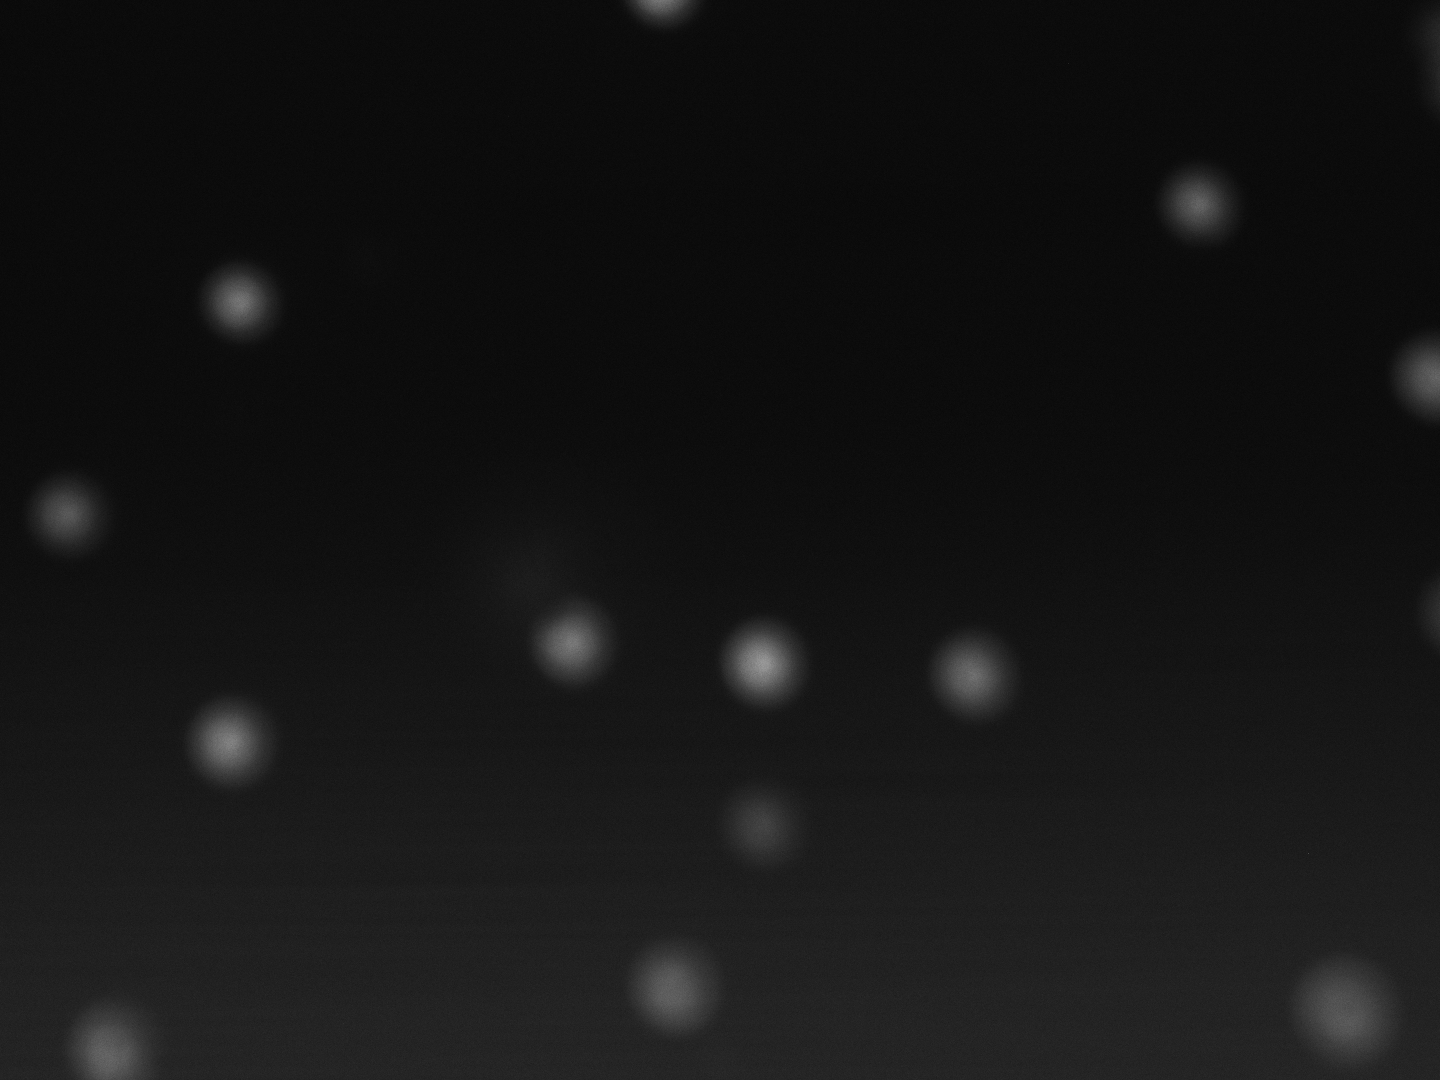
\includegraphics[width=\textwidth]{essai_10um_2im_100ms.png}
    \caption{Échantillon avec particules de 10 µm}
  \end{subfigure}
  \hfill
  \begin{subfigure}[H]{0.45\textwidth}
    \centering
    \includegraphics[width=\textwidth]{Échantillon1um.png}
    \caption{Échantillon avec particules de 1 µm}
  \end{subfigure}
  \caption{Images d'échantillons testés pour comparaison qualitative}
\end{figure}

\subsection{Résolution de l'instrument}

La résolution de l'instrument concernant la taille des particules observables est définie
comme la plus petite différence qu'il est capable de discerner. Selon les tests effectués, 
cette plus petite différence est obtenue lors de l'identification des particules de 1 um 
de diamètre. Elle correspond à l'incertitude obtenue sur la valeur estimée, ce qui se traduit
par une résolution de 0,3 um. 

\subsection{Limitations de l'appareil}

L'appareil peut distinguer et suivre des particules dans la gamme de 1 à 10 um avec et sans dérive.
Toutefois, pour estimer la taille des particules, une dérive trop forte peut affecter négativement 
les performances de l'appareil. La grande dérive des particules dans l'échantillon de particules 
de 10 um est la raison pour laquelle leur étude statistique n'est faite qu'avec 3 données, puisque 
les tests effectués avec les autres particules de l'échantillon ne permettaient pas d'obtenir une 
valeur cohérente. La valeur obtenue était soit négative, soit erronée par plusieurs ordres de grandeur.

Un seuil critique survient lorsque la dérive est de quelques ordres de grandeur supérieure à la 
diffusion associée au mouvement brownien. Dans ce régime, malgré une 
compensation de la plus grande partie de la dérive, l'incertitude qu'elle vient ajouter, bien que faible
relativement au mouvement de dérive, est grande par rapport à la diffusion. Celle-ci n'est alors plus 
adéquatement estimée par le modèle utilisé. L'autre facteur qui semble ici déterminant est l'angle de la
dérive qui ne semble pas être constant. Cette dérive non-homogène dans l'espace échappe alors en partie
à la suppression du coefficient quadratique et ses composantes viennent renforcer le déplacement latéral
attribué à la diffusion, ce qui augmente la mobilité de la particule et fausse les résultats. 

Il y a plusieurs sources potentielles pour ces types de dérive. D'abord, pour la grande dérive, une 
fuite due à un mauvais calfeutrage de l'échantillon peut causer un 




\subsection{Étude des coûts}

Une étude des coûts a été faite pour le microscope construit afin de voir s'il y a possibilité
de construire un appareil aux performances similaires, mais à moindre coût. Le tableau \ref{table_cout}
présente la liste exhaustive des pièces avec leur prix en dollars canadiens avant taxes.

\begin{table}[!ht]
    \centering
    \caption{Liste des pièces et coûts totaux pour le microscope sur table optique
    \cite{noauthor_thorlabs_2024} \cite{noauthor_m-tsx-1d_2024}.}
    \begin{tabular}{|l|l|l|l|l|}
    \hline
        ID pièce & Description & Qté & \$ CAD & Total ind. \\ \hline\hline
        KM100S & Montage ajustable pour échantillon & 1 & \$130.45 & \$130.45 \\ \hline
        M-TSX-1S & Platine de translation & 1 & \$305.80 & \$305.80 \\ \hline
        CS165MU & Caméra CMOS monochrome & 1 & \$667.01 & \$667.01 \\ \hline
        - & Objectif de microscope & 1 & \$10.00 & \$10.00 \\ \hline
        420FDL12 & Filtre passe-long & 1 & \$36.29 & \$36.29 \\ \hline
        LA1433-A-ML & Lentille tube f = 150.0 mm & 1 & \$71.42 & \$71.42 \\ \hline
        CPS405 & Laser bleu 405 nm & 1 & \$312.07 & \$312.07 \\ \hline
        LMR1 & Trou taraudé pour lentilles & 2 & \$22.89 & \$45.79 \\ \hline
        TR3-P5 & 5 tiges 3 po pour optiques & 1 & \$38.50 & \$38.50 \\ \hline
        PH4 & Base pour tiges d'optique 4 po & 4 & \$14.83 & \$59.33 \\ \hline
        PH3 & Base pour tiges d'optique 3 po & 1 & \$13.37 & \$13.37 \\ \hline
        BA1 & Pied de montage optique & 1 & \$8.42 & \$8.42 \\ \hline
        BA1S & Pied de montage optique & 2 & \$7.83 & \$15.65 \\ \hline
        BA2 & Pied de montage optique & 1 & \$11.26 & \$11.26 \\ \hline
        VC1 & Pince en V & 1 & \$64.04 & \$64.04 \\ \hline\hline
        ~ & ~ & ~ & Total : & \$1789.39 \\ \hline
    \end{tabular}
    \label{table_cout}
\end{table}

% Source Thorlabs : https://www.thorlabs.com
% Source Platine : https://www.newport.com/p/M-TSX-1D

Quelques éléments sont à souligner. Premièrement, étant donné que l'objectif de microscope a
été fourni par le gouvernement du Québec, le coût qui y est associé a été estimé selon leurs
informations. Ces objectifs sont de seconde main, et ils ont été achetés en ensemble. Cela mène
au faible coût d'environ 10\$, qui pourrait être difficile à retrouver pour la construction d'un
seul microscope. Toutefois, pour la construction d'un ensemble d'appareils spécialisés pour
différentes tailles de particules, donc ayant besoin de différents objectifs à différents 
grossissements, le prix d'ensemble est idéal. Deuxièmement, un coût important a été omis dans 
le tableau de calcul, soit celui de la table optique elle-même. Cette dernière est très
dispendieuse, mais elle a été omise, car elle est déjà présente dans plusieurs laboratoires 
d'optique, ou si non, elle peut être acheté à plus faible coût si les dimensions de la table
achetée se limitent aux dimensions de l'appareil. Par exemple, chez Thorlabs, la plus petite 
table optique pour tenir ce microscope est la B1824F, avec des dimensions de 18" $\times$ 24" \cite{noauthor_thorlabs_2024}.
Avec un coût de 1319.08 CAD, presque l'entièreté du coût du reste de l'appareil, le total
monte à 3108.47 \$. Troisièmement, selon le tableau \ref{table_cout}, les pièces ayant les
coûts les plus considérables sont celles directement liées à l'optique et à l'alignement. Le
reste des pièces sont pour des éléments de construction du montage, et leur total s'élève à
1039.11 \$.

Il est donc possible de recommander fortement l'utilisation de l'impression 3D pour une production
à plus grand volume de ce microscope. Cela permettra de sauver l'argent sur les pièces de
construction et sur la table optique elle-même, aiderait à l'alignement des éléments optiques,
permettrait plus de flexibilité sur les composantes à ajuster tel que le montage de l'échantillon pour
s'occuper du focus, et enfin pourrait rendre l'appareil plus portatif pour des essais sur le terrain.
Comme les éléments optiques seraient tous réutilisables dans un design d'impression 3D, les
performances du dispositif resteraient identiques. Il est aussi possible de recommander l'usage
d'un différent laser de 405 nm, car ils sont fréquemment vendus en seconde main pour beaucoup moins
cher.

\section{Annexes}

\subsection{Programme de prise de données avec la caméra}

\begin{lstlisting}[language=python]
import numpy as np
import matplotlib as plt
import pycromanager
from pycromanager import Core
import time
from typing import Any
from PIL import Image
import pylablib as pll
from pylablib.devices import Thorlabs
from thorlabs_tsi_sdk.tl_camera import TLCameraSDK, OPERATION_MODE, TLCameraError

pll.par["devices/dlls/thorlabs_tlcam"] = r"C:\Users\marie\Documents\Scientific Camera Interfaces\SDK\Python Toolkit\dlls\64_lib"

#Numero de serie de la camera
print(Thorlabs.list_cameras_tlcam())

try:
    # Initialiser le SDK
    sdk = TLCameraSDK()
    print("SDK initialise avec succes.")

    # Decouvrir les cameras disponibles
    available_cameras = sdk.discover_available_cameras()
    print(f"Cameras disponibles : {available_cameras}")

    if not available_cameras:
        print("Aucune camera trouvee. Verifiez la connexion.")
        sdk.dispose()
        exit()

    # Essayer d'ouvrir la premiere camera disponible
    try:
        with sdk.open_camera(available_cameras[0]) as cam1:
            print(f"Camera connectee avec succes : {available_cameras[0]}")

            # Configurer les parametres de la camera
            cam1.exposure_time_us = 125000  # Exemple de temps d'exposition de 50 ms (tester sur Thorlab)
            cam1.black_level=1
            cam1.gain=0
            cam1.frames_per_trigger_zero_for_unlimited = 1  # Mode de capture continue : 0 ; Mode de capture ponctuel : 1
            cam1.arm(10)  # Preparez la camera avec 2 tampons
            nombre_image_par_seconde=2
            print("Camera armee et prete pour capturer des images.")
            
            output_tiff_path = r"C:\Users\marie\Documents\GitHub\super_res_microscopy\acquisition\video_output_carac_125ms_2im_poussieres.tiff"

            # Capture and save images
            images = []  # List to store frames for TIFF
            for picture_number in range(5):  # Capture 100 frames
                cam1.issue_software_trigger()
                time.sleep(1 / nombre_image_par_seconde)  # Maintain frame rate

                frame = cam1.get_pending_frame_or_null()
                if frame is not None:
                    print(f"Image successfully captured: {frame.frame_count}")
                    # Convert the image buffer to a NumPy array
                    image = np.array(frame.image_buffer, dtype=np.uint8).reshape(
                        (cam1.image_height_pixels, cam1.image_width_pixels)
                    )
                else:
                    image = np.zeros((cam1.image_height_pixels, cam1.image_width_pixels), dtype=np.uint8)
                    print("No image captured.")

                # Add the image to the list as a Pillow Image
                images.append(Image.fromarray(image))

            # Save all frames as a multi-page TIFF
            if images:
                images[0].save(
                    output_tiff_path,
                    save_all=True,
                    append_images=images[1:],  # Save as multi-page TIFF
                    compression="tiff_deflate"  # Optional: Apply compression
                )
                print(f"Multi-page TIFF saved at: {output_tiff_path}")
            else:
                print("No frames to save.")

            # Desarmer et fermer la camera apres utilisation
            cam1.disarm()
            print("Camera desarmee et fermee.")


    except TLCameraError as e:
        print(f"Erreur lors de la connexion de la camera : {e}")
        print("Verifiez que la camera est correctement connectee et non utilisee par un autre programme.")

    finally:
        # Assurez-vous que le SDK est libere pour liberer les ressources
        sdk.dispose()

except TLCameraError as e:
    print(f"Erreur SDK : {e}")

finally:
    # Nettoyer le SDK correctement
    if 'sdk' in locals():
        sdk.dispose()
\end{lstlisting}

\subsection{Programme d'analyse des particules de 1 micron}

\begin{lstlisting}[language=python]
import matplotlib
matplotlib.use('Qt5Agg')  # Utiliser le backend Qt5Agg pour Windows
import matplotlib.pyplot as plt
import matplotlib.animation as animation
from scipy.optimize import curve_fit
import cv2
import numpy as np
import os
from PIL import Image
import lmfit
#import tifffile
#%matplotlib tk #pour Linux

import scipy.ndimage as ndimage
from sklearn.cluster import DBSCAN

path_to_tiff = os.path.join("..", "acquisition", "essai_10um_2im_50ms.tiff")
tiff = Image.open(path_to_tiff)

with Image.open(path_to_tiff) as img:
    frame_number = 0
    actual_frames = 0
    try:
        while True:
            frame_number += 1
            if np.sum(np.array(img)) != 0:
                actual_frames += 1
                
            img.seek(frame_number)
    except EOFError:
        print("All frames processed.")

frame_index = 0
first_frame = 0
tiff.seek(frame_index)
original_image = np.array(tiff)

while np.sum(original_image) == 0:
    frame_index += 1
    tiff.seek(frame_index)
    original_image = np.array(tiff)
    first_frame += 1
    print(frame_index)

clahe = cv2.createCLAHE(clipLimit=10.0, tileGridSize=(30, 30))
preprocessed = clahe.apply(original_image)

blurred = cv2.medianBlur(preprocessed, 115)
preprocessed2 = cv2.subtract(preprocessed, blurred)

# Apply Non-Local Means Denoising
img = cv2.fastNlMeansDenoising(preprocessed2, None, 15, 7, 41)

def crop(img, x, y, crop_size_x, crop_size_y):  
    x_start = int(x - crop_size_x // 2)
    x_end = int(x + crop_size_x // 2)
    y_start = int(y - crop_size_y // 2)
    y_end = int(y + crop_size_y // 2)

    if x_start < 0:
        x_start = 0
    if x_end > 1440:
        x_end = 1440
    if y_start < 0:
        y_start = 0
    if y_end > 1080:
        y_end = 1080

    return img[y_start:y_end, x_start:x_end]

fig, ax = plt.subplots()
ax.imshow(img, origin='lower', cmap='gray')
plt.title(f"Frame {frame_index}: Select a point")

# Selection de points
print("Please click on the point you want to select.")
x, y = plt.ginput(1)[0] 
print(f"Selected point: ({x}, {y})")
plt.close()

crop_sze_x = 250
crop_sze_y = 300

def visionneur(frame, titre):
    plt.figure(figsize=(10, 5))
    plt.clf() 
    plt.imshow(frame, origin='lower', cmap='gray')
    plt.title(titre)
    plt.colorbar()  
    plt.show()

def prepare_data(x, y, z):
    return (x.flatten(), y.flatten()), z.flatten()

def gaussian_2d(xy, amplitude, x0, y0, sigma_x, sigma_y, offset):
    x, y = xy
    a = 1 / (2 * sigma_x**2)
    b = 1 / (2 * sigma_y**2)
    return offset + amplitude * np.exp(- (a * (x - x0)**2 + b * (y - y0)**2))

def localisateur_gaussien(intensity_grid, centre):
    x = np.arange(intensity_grid.shape[1])
    y = np.arange(intensity_grid.shape[0])
    X, Y = np.meshgrid(x, y)

    # Preparer les donnees pour le fit
    (xdata, ydata), zdata = prepare_data(X, Y, intensity_grid)
    model = lmfit.Model(gaussian_2d)
    max_idx = np.unravel_index(np.argmax(intensity_grid), intensity_grid.shape)

    initial_x0 = x[max_idx[1]]
    initial_y0 = y[max_idx[0]]

    # Definir les parametres du modele
    params = model.make_params(
        amplitude=np.max(intensity_grid),
        x0=initial_x0,
        y0=initial_y0,
        sigma_x=5,
        sigma_y=5,
        offset=3
    )

    # Ajouter des bornes sur les parametres x0 et y0
    params['x0'].min = 0    # Limite inferieure pour x0
    params['x0'].max = intensity_grid.shape[1] - 1  # Limite superieure pour x0
    params['y0'].min = 0    # Limite inferieure pour y0
    params['y0'].max = intensity_grid.shape[0] - 1  # Limite superieure pour y0

    # Ajouter des bornes sur les parametres sigma
    params['sigma_x'].min = 1  # Limite inferieure de sigma_x
    params['sigma_x'].max = 40 # Limite superieure de sigma_x
    params['sigma_y'].min = 1  # Limite inferieure de sigma_y
    params['sigma_y'].max = 40 # Limite superieure de sigma_y

    # Effectuer l'ajustement
    result = model.fit(zdata, params, xy=(xdata, ydata))
    
    x_position = result.params['x0'].value + centre[0] - crop_sze_x//4
    y_position = result.params['y0'].value + centre[1] - crop_sze_y//4

    return [x_position, y_position], result.params['sigma_x'].value, result.params['sigma_y'].value

def denoise(image):
    clahe = cv2.createCLAHE(clipLimit=10.0, tileGridSize=(30, 30))
    preprocessed = clahe.apply(image)
    
    blurred = cv2.medianBlur(preprocessed, 115)
    preprocessed2 = cv2.subtract(preprocessed, blurred)
    
    return cv2.fastNlMeansDenoising(preprocessed2, None, 15, 7, 41)

def is_within_bounds(position):
    x, y = position

    # Definir les bornes du cadre
    x_min, x_max = 100, 1300
    y_min, y_max = 100, 980

    # Verifier si la position est dans les bornes du cadre
    if x_min <= x <= x_max and y_min <= y <= y_max:
        return True
    else:
        return False

def empreinte_digitale(image, threshold=50, eps=3, min_samples=1):
    # 1. Observer chaque particule approximativement
    visionneur(image, f'particule choisie')

    maxima = (image > threshold)
    
    coordinates = np.column_stack(np.where(maxima))  
    if coordinates.shape[0] == 0:
        print("Aucune particule detectee.")
        return [], image

    dbscan = DBSCAN(eps=eps, min_samples=min_samples)
    labels = dbscan.fit_predict(coordinates)
    unique_labels = np.unique(labels)
    size=0

    # 2. Determiner l'empreinte digitale de notre particule
    for label in unique_labels:
        if label != -1:  # -1 correspond au bruit dans DBSCAN
            cluster_points = coordinates[labels == label]
            plt.scatter(cluster_points[:, 1], cluster_points[:, 0], label=f'Particule {label}')

            if cluster_points.shape[0]>size:
                size = cluster_points.shape[0]
                luminosity = np.mean(image[cluster_points[:, 0], cluster_points[:, 1]])

    seuil=np.max(image)*0.5
    print(f'seuil:{seuil}, taille:{size} et luminosite: {luminosity}')

    # 3. Afficher les resultats et filtrer les particules selon leur taille et luminosite
    plt.imshow(image, origin='lower', cmap='gray')
    plt.title(f"Empreinte digitale de la particule, lum={luminosity} et taille={size}")
    plt.legend()
    plt.colorbar()  
    plt.show()

    return size, luminosity, seuil

def detect_nbre_particles(image, threshold, eps=9, min_samples=1):
    # 1. Appliquer un filtre de voisinage pour detecter les maxima locaux
    neighborhood_size = 3  # Taille du voisinage pour detecter les maxima locaux
    local_max = ndimage.maximum_filter(image, size=neighborhood_size)
    # 2. Comparer l'image originale et les maxima locaux pour identifier les vrais maxima
    maxima = (image == local_max) & (image > threshold)

    # 3. Extraire les coordonnees des maxima (particules)
    coordinates = np.column_stack(np.where(maxima))  # Extraire les indices des pixels maximaux
    if coordinates.shape[0] == 0:
        print("Aucune particule detectee.")
        visionneur(image, f'detection du nombre de particules')

        return [], image

    # 4. Appliquer DBSCAN pour regrouper les particules proches (cluster les maxima detectes)
    dbscan = DBSCAN(eps=eps, min_samples=min_samples)
    labels = dbscan.fit_predict(coordinates)

    #5. Determiner le nombre de particules
    unique_labels = np.unique(labels)
    nb_particules = len(unique_labels)
        
    positions=[]
    for label in unique_labels:
        if label != -1:  # -1 correspond au bruit dans DBSCAN
            cluster_points = coordinates[labels == label]
        positions.append((np.mean(cluster_points[:, 1]), np.mean(cluster_points[:, 0])))

    # Retourner les coordonnees des particules filtrees
    return nb_particules, positions

def identificateur_particles(image, ref_size, ref_luminosity, threshold=50, eps=9, min_samples=1):
    # 1. Obtenir le plus d'info sur la particule
    maxima = (image > threshold)
    
    coordinates = np.column_stack(np.where(maxima))  
    if coordinates.shape[0] == 0:
        print("Mauvais re-crop empeche identification de la particule.")
        return [], image

    dbscan = DBSCAN(eps=eps, min_samples=min_samples)
    labels = dbscan.fit_predict(coordinates)
    unique_labels = np.unique(labels)

    # 2. Parcourir chaque particule et identifier laquelle est celle qu'on suit
    distances = []
    position_particules = []

    for label in unique_labels:
        if label != -1:  # -1 correspond au bruit dans DBSCAN
            cluster_points = coordinates[labels == label]
            plt.scatter(cluster_points[:, 1], cluster_points[:, 0], label=f'Particule {label}')

            size = cluster_points.shape[0]
            luminosity = np.mean(image[cluster_points[:, 0], cluster_points[:, 1]])
            size_distance = abs(size - ref_size)  
            luminosity_distance = abs(luminosity - ref_luminosity) 
            
            combined_distance = size_distance + luminosity_distance
            distances.append(combined_distance)
            position_particules.append((np.mean(cluster_points[:, 1]), np.mean(cluster_points[:, 0])))

    ecart = np.min(distances)
    position_best_particle = position_particules[np.argmin(distances)]  

    return position_best_particle, ecart

def particle_tracker_simple(image, x, y):
    image = denoise(image)

    cropped_img = crop(image, x, y, crop_sze_x, crop_sze_y)
    
    #Gerer plus qu'une particule
    cropped_img = np.array(cropped_img)
    max_index = np.argmax(cropped_img)
    max_coords = np.unravel_index(max_index, cropped_img.shape)

    nouveau_x = x - crop_sze_x // 2 + max_coords[1]
    nouveau_y = y - crop_sze_y // 2 + max_coords[0]
    
    second_crop = crop(image, nouveau_x, nouveau_y, crop_sze_x, crop_sze_y)    # Re-crop autour d'une seule particule

    result_fit = localisateur_gaussien(second_crop, [nouveau_x, nouveau_y])

    x_new, y_new = result_fit[0][0], result_fit[0][1]

    return [result_fit, cropped_img, (x_new, y_new), (result_fit[1], result_fit[2])]

#Places ici pour pouvoir y faire reference dans particule_tracker
position_list=[[x,y]]
sigma_list = []
crop_frames = []
big_frames = []

def particle_tracker(imge, x, y, taille_initiale, luminosite_initiale, seuil):
    # 1. Ce qu'on voit pres de l'ancienne position
    image = denoise(imge)

    cropped_img = crop(image, x, y, crop_sze_x, crop_sze_y)
    
    # 2. Determiner combien il y a de particules et laquelle est la notre
    # Utiliser une reconnaissance de particules et si plus qu'une, alors clic pour choisir
    nb_part, coordonnees = detect_nbre_particles(cropped_img, seuil)

    if nb_part == 1:
        cropped_img = np.array(cropped_img)
        max_index = np.argmax(cropped_img)
        max_coords = np.unravel_index(max_index, cropped_img.shape)

        nouveau_x = x - crop_sze_x // 2 + max_coords[1] #Oui c'est inverse a cause du unravel juste avant
        nouveau_y = y - crop_sze_y // 2 + max_coords[0]
    elif  (nb_part == 0) or (nb_part == []):
        # choix de point
        fig, ax = plt.subplots()
        ax.imshow(denoise(img), origin='lower', cmap='gray') 
        plt.title(f"Frame {len(position_list)-1}: Select a point")

        # Ajouter une croix rouge a la position donnee
        cx, cy = position_list[len(position_list)-1]
        ax.plot(cx, cy, 'rx', markersize=10) 
        
        # Afficher l'image et demander a l'utilisateur de cliquer
        print("Please click on the point you want to select.")
        nouveau_x, nouveau_y = plt.ginput(1)[0]  # Attente du clic de l'utilisateur (1 point)
        
        # Fermer l'affichage apres selection
        plt.close()
    else:
        imperfections, emplacements = [] , []
        for num_particule in range(nb_part):
            x_identifier=x - crop_sze_x // 2 + coordonnees[num_particule][0]
            y_identifier=y - crop_sze_y // 2 + coordonnees[num_particule][1]
            crop_pour_identifier = crop(image, x_identifier, y_identifier, crop_sze_x//2, crop_sze_x//2)
            emplacement, ecart = identificateur_particles(crop_pour_identifier, taille_initiale, luminosite_initiale, seuil)
            imperfections.append(ecart)
            emplacements.append(emplacement)
        qualite = np.min(imperfections)
        print(f'ecart:{qualite}')
        max_coords = emplacements[np.argmin(imperfections)]  
        nouveau_x = x_identifier - crop_sze_x // 4 + max_coords[0]
        nouveau_y = y_identifier - crop_sze_y // 4 + max_coords[1]
    
    # Verification s'il fout le camp 
    dis = np.sqrt((position_list[-1][0]-nouveau_x)**2+(position_list[-1][1]-nouveau_y)**2)
    if dis>100:
        # Display the image and let the user select a point interactively
        fig, ax = plt.subplots()
        ax.imshow(denoise(img), origin='lower', cmap='gray') 
        plt.title(f"Frame {len(position_list)-1}: Probleme d'identification, nouvelle pos a {dis}, select a point")

        print('probleme d''identification')
        # Ajouter une croix rouge a la position donnee
        cx, cy = position_list[-1]
        ax.plot(cx, cy, 'rx', markersize=10) 
        
        # Afficher l'image et demander a l'utilisateur de cliquer
        print("Please click on the point you want to select.")
        nouveau_x, nouveau_y = plt.ginput(1)[0]  # Attente du clic de l'utilisateur (1 point)
        print(f"Selected point: ({nouveau_x}, {nouveau_y})")
        
        # Fermer l'affichage apres selection
        plt.close()
    
    # 3. Crop autour de notre particule et fit dessus
    second_crop = crop(image, nouveau_x, nouveau_y, crop_sze_x//2, crop_sze_y//2)    # Re-crop autour d'une seule particule

    result_fit = localisateur_gaussien(second_crop, [nouveau_x, nouveau_y])

    x_new, y_new = result_fit[0][0], result_fit[0][1]

    return [result_fit, second_crop, (x_new, y_new), (result_fit[1], result_fit[2])]

taille_initiale, luminosite_initiale, seuil = empreinte_digitale(crop(img,x,y,crop_sze_x*0.8,crop_sze_y*0.5))
print(f'position initiale: {position_list}')

for i in range(first_frame,actual_frames):
    tiff.seek(i)
    if np.sum(np.array(tiff))==0:
        position_list.append(np.array([np.nan,np.nan]))
        sigma_list.append(np.array([np.nan,np.nan]))
        print(f'frames vide:{i}')
    else:
        data = particle_tracker(img, x, y, taille_initiale, luminosite_initiale, seuil)
        position_list.append(data[2])
        x,y = position_list[i-first_frame+1]
        sigma_list.append(data[3])
        tiff.seek(i)
        img = np.array(tiff)
        big_frames.append(img)
        crop_frames.append(data[1])
        if is_within_bounds(position_list[-1]):
            pass
        else:
            break
    print(f'liste des positions frame {i}:{position_list}')

pixel_size = 3.45 # Taille absolue
f2 = 150  # Focale de L2
M_theo = 20  # Magnification
pxl = pixel_size / (f2 * M_theo / 160)  # Pixel size en um dans le plan de la particule

sigma_arr=np.array(sigma_list)* pxl * 10**(-6)
position_arr=np.array(position_list)* pxl * 10**(-6)
print(position_arr)

def calculate_msd_with_uncertainty(position_arr, delta_x, delta_y):
    """
    Calcule les MSD avec propagation des incertitudes analytiques.
    """
    if position_arr[0:].shape[0] != delta_x[0:].shape :
        position_arr=position_arr[:len(position_arr)-1]

    # Traitement Lucien
    diff_pair = np.zeros_like(position_arr[1:])
    dx = np.zeros_like(delta_x[1:])
    dy = np.zeros_like(delta_y[1:])

    # Masque pour detecter les NaN
    nan_mask_pos = np.isnan(position_arr[1:]) | np.isnan(position_arr[:-1])
    nan_mask_delta = np.isnan(delta_x[1:]) | np.isnan(delta_x[:-1])
    
    # Calculer les differences uniquement ou nan_mask est False
    valid_mask_pos = ~nan_mask_pos.any(axis=1)  # Inverser le masque pour obtenir les position_arr valides
    valid_mask_delta = ~nan_mask_delta
    
    diff_pair[valid_mask_pos] = position_arr[1:][valid_mask_pos, :] - position_arr[:-1][valid_mask_pos, :]
    # Calculer les differences en x uniquement (prendre la premiere colonne des positions)
    print(len(diff_pair))
    vitesse_moyenne = np.mean(diff_pair,axis=0)
    
    temps = np.arange(0,len(position_arr))  # vecteur de temps

    # Appliquer la soustraction terme a terme
    nouvelles_donnees = position_arr - vitesse_moyenne * temps[:, np.newaxis]    
    print(f'vitesse moyenne d'f'environ: {vitesse_moyenne}')
    
    msd = []
    uncertainties = []
    for d in range(1, len(nouvelles_donnees)):
        diff_pairs = np.zeros_like(nouvelles_donnees[d:])
        dx = np.zeros_like(delta_x[d:])
        dy = np.zeros_like(delta_y[d:])

        # Masque pour detecter les NaN
        nan_mask_pos = np.isnan(nouvelles_donnees[d:]) | np.isnan(nouvelles_donnees[:-d])
        nan_mask_delta = np.isnan(delta_x[d:]) | np.isnan(delta_x[:-d])
        
        # Calculer les differences uniquement ou nan_mask est False
        valid_mask_pos = ~nan_mask_pos.any(axis=1)  # Inverser le masque pour obtenir les position_arr valides
        valid_mask_delta = ~nan_mask_delta
        
        diff_pairs[valid_mask_pos] = nouvelles_donnees[d:][valid_mask_pos, :] - nouvelles_donnees[:-d][valid_mask_pos, :]

        distances_squared = np.sum(diff_pairs**2, axis=1)
        msd.append(np.mean(distances_squared))  
        
        dx[valid_mask_delta] = delta_x[d:][valid_mask_delta] + delta_x[:-d][valid_mask_delta]
        dy[valid_mask_delta] = delta_y[d:][valid_mask_delta] + delta_y[:-d][valid_mask_delta]
        term_x = 2 * (diff_pairs[:, 0]**2) * (dx**2)
        term_y = 2 * (diff_pairs[:, 1]**2) * (dy**2)

        # Propagation des incertitudes
        total_uncertainty = np.mean(term_x + term_y)
        uncertainties.append(np.sqrt(total_uncertainty))

    return np.array(msd), np.array(uncertainties)

calculate_msd_with_uncertainty(position_arr, sigma_arr[:, 0], sigma_arr[:, 1])

msd_values, uncertainties = calculate_msd_with_uncertainty(position_arr, sigma_arr[:, 0], sigma_arr[:, 1])

time_intervals = np.arange(1, len(msd_values) + 1) * 0.5

# Plot MSD
plt.figure(figsize=(8, 6))
plt.errorbar(time_intervals, msd_values, yerr=uncertainties, fmt='o', label='MSD', color='blue')
plt.title("MSD en fonction de l'intervalle de temps")
plt.xlabel("Intervalle de temps")
plt.ylabel("MSD")
plt.grid(True)
plt.legend()
plt.show()

# Fonction quadratique pour l'ajustement
def quadratic(x, a, b, c):
    return a * x**2 + b * x + c
def line(x, b,c):
    return b*x+c

msd_values, uncertainties = calculate_msd_with_uncertainty(position_arr, sigma_arr[:, 0], sigma_arr[:, 1])

cropped_msd = msd_values[:5]
cropped_inc = uncertainties[:5]

time_intervals = np.arange(1, len(cropped_msd) + 1)

# curve fit quadratique
bounds = ([-np.inf, -np.inf, -np.inf], [np.inf, np.inf, np.inf])
popt, pcov = curve_fit(line, time_intervals, cropped_msd, sigma=cropped_inc)

# coefficients optimaux
coeffs = popt

  # Incertitudes sur les coefficients sont les elements diagonaux
coeff_uncertainties = np.sqrt(np.diag(pcov))

# Affichage des coefficients separement
print("Coefficients du polynome ajuste :")
print(coeffs)

# Affichage de la matrice de covariance separement
print("Matrice de covariance des coefficients :")
print(pcov)

# Creation de la fonction quadratique de l'ajustement
quadratic_fit = np.poly1d(coeffs)

# Generation des valeurs ajustees pour afficher la courbe
fitted_msd = quadratic_fit(time_intervals)

# Affichage du MSD avec les barres d'erreur
plt.figure(figsize=(8, 6))
plt.errorbar(time_intervals, cropped_msd, yerr=cropped_inc, fmt='o', label='MSD', color='blue')
plt.plot(time_intervals, fitted_msd, label='Quadratic Fit', color='red', linestyle='--')
plt.title("MSD en fonction de l'intervalle de temps")
plt.xlabel("Intervalle de temps")
plt.ylabel("MSD")
plt.grid(True)
plt.legend()
plt.show()

# Affichage des incertitudes sur les coefficients
print(f"Incertitudes sur les coefficients : {coeff_uncertainties}")

# Calcul du coefficient de diffusion et de la taille de la particule
r = (4 * 1.38 * 10**-23 * 300 / (6 * np.pi * 10**(-3) * coeffs[0]))  # Coefficient de diffusion
r_uncertainty = (4 * 1.38 * 10**(-23) * 300 * coeff_uncertainties[0] / (6 * np.pi * 10**(-3) * (coeffs[0])**2))  # Coefficient de diffusion

# Affichage de la taille de la particule avec incertitude
print(f"Taille de la particule (m): {r:.2e} m, avec une incertitude : {r_uncertainty:.2e}")
\end{lstlisting}

\subsection{Preuve de correction par Antidote}
\begin{figure}[H]
  \centering
  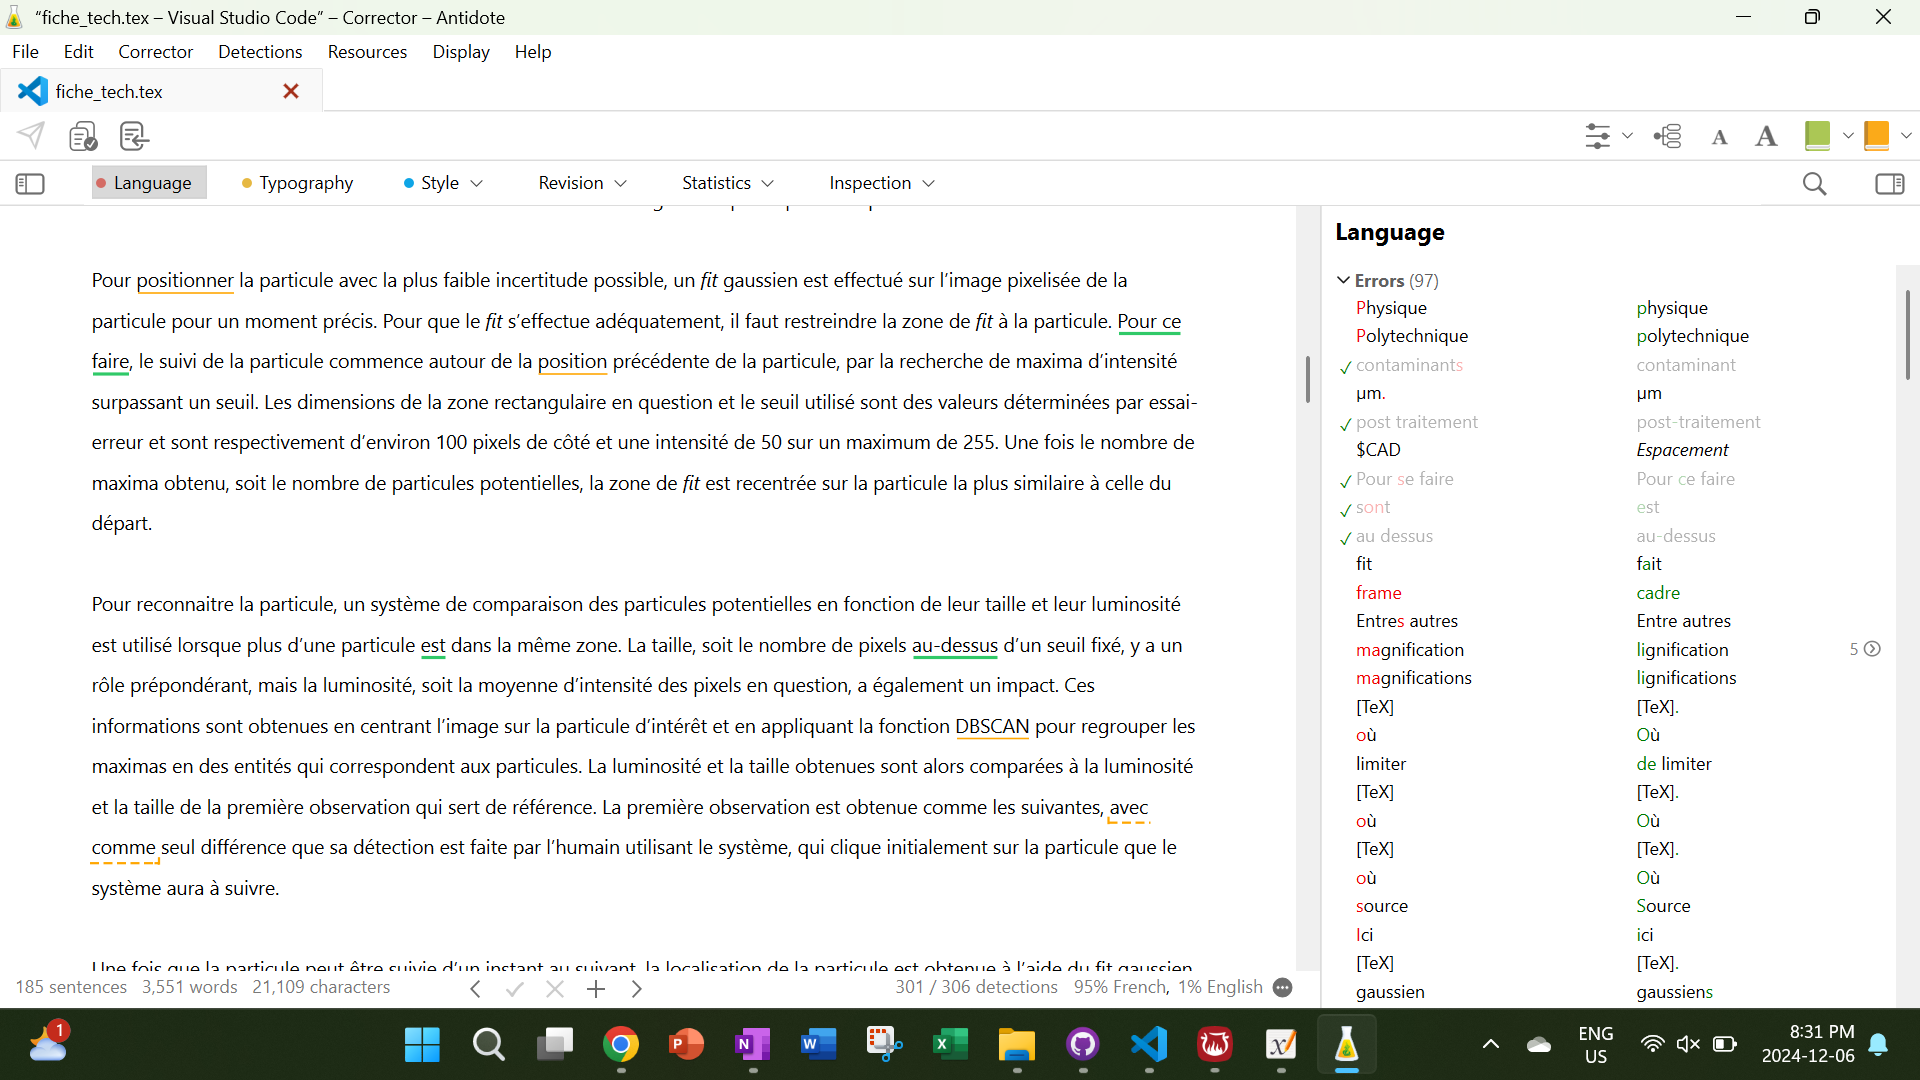
\includegraphics[scale=0.2]{Screenshot (1).png}
  \caption{Correction par Antidote}
\end{figure}
\clearpage

\bibliographystyle{unsrtnat}
\bibliography{suivi_particules.bib}



\end{document}
